\begin{frame}{Git vs SVN}
\begin{itemize}
  \item Git is a fully distributed version control system (VCS)
  \item Each user (PC/Laptop) is an exact clone of the remote repository
    \begin{itemize}
      \item Each user is a repository (log, revert, merge, branch, etc)
      \item No network connection required, except to sync with central repo (pull/push/fetch)
      \item merge and rebasing can be done offline
    \end{itemize}
  \item Git is much faster than SVN
  \item Git's repositories are much smaller than SVN
  \item Git's branches are much simpler and less resource heavy than SVN
  \item Git is much better in branch auditing and merge handling
  \item As many backups as the number of users
  \item Content integrity using SHA-1 hash
  \end{itemize}
\end{frame}

\begin{frame}{Git vs SVN}
  \begin{figure}
    \begin{center}
    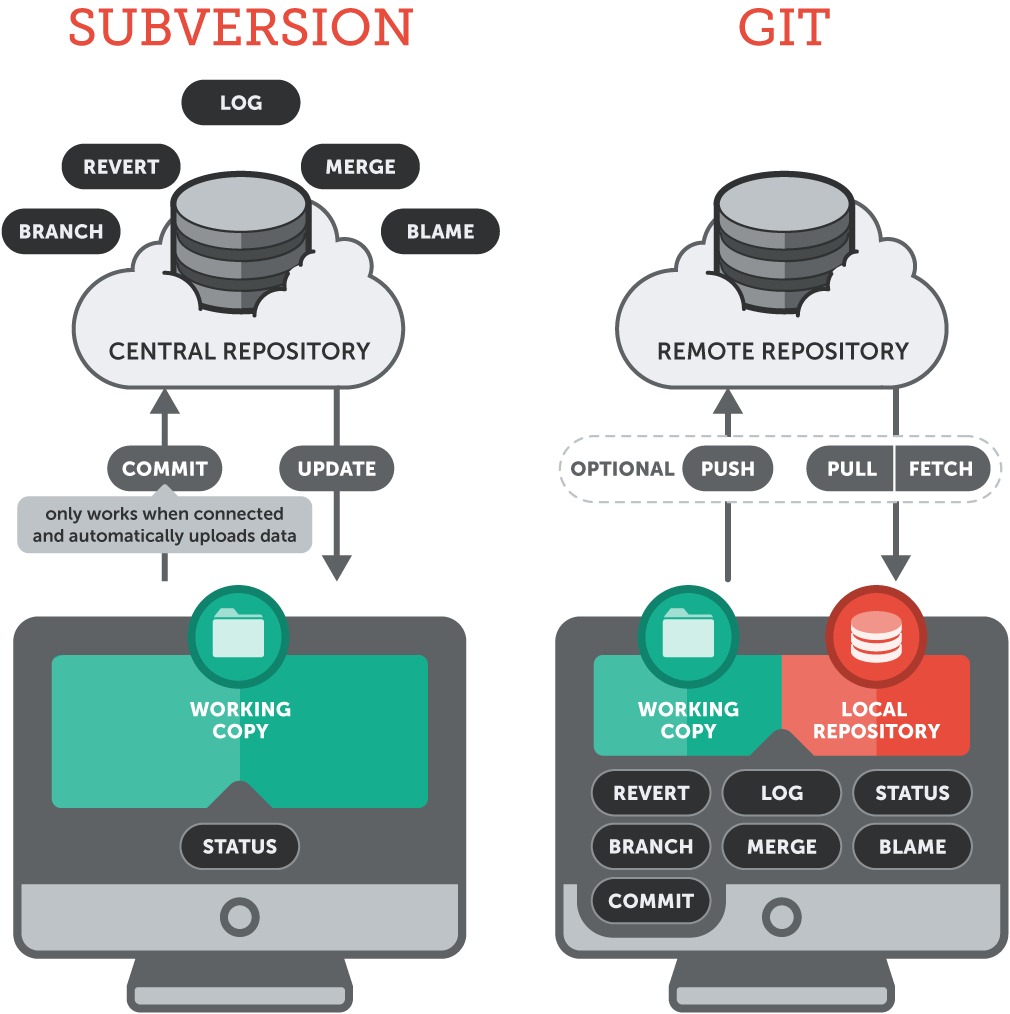
\includegraphics[width=0.5\linewidth]{pics/git-vs-svn.png}
    \vspace{-0.3cm}
    \caption{\footnotesize Centralized vs distributed VCS (Source: www.git-tower.com)}
  \end{center}
\end{figure}
\end{frame}

\begin{frame}{Git vs SVN}
  \begin{center}
  \begin{tabular}{ c || c | c  }
         & SVN & Git \\ \hline\hline
    \textbf{License} & Open-source (Apache) & GNU \\
    \textbf{Distributed-ness} & Centralized & Fully Distributed  \\
    \textbf{Speed} & \Cross & \Check \\
    \textbf{Storage} & \Cross & \Check \\
    \textbf{Integrity Guarantee} & \Cross & \Check \\
    \textbf{Brnaching \& merging} & \Cross & \Check \\
    \textbf{Stashing} & \Cross & \Check \\

      \end{tabular}
    \end{center}
\end{frame}

